% Options for packages loaded elsewhere
\PassOptionsToPackage{unicode}{hyperref}
\PassOptionsToPackage{hyphens}{url}
%
\documentclass[
  12pt,
  ignorenonframetext,
]{beamer}
\usepackage{pgfpages}
\setbeamertemplate{caption}[numbered]
\setbeamertemplate{caption label separator}{: }
\setbeamercolor{caption name}{fg=normal text.fg}
\beamertemplatenavigationsymbolsempty
% Prevent slide breaks in the middle of a paragraph
\widowpenalties 1 10000
\raggedbottom
\setbeamertemplate{part page}{
  \centering
  \begin{beamercolorbox}[sep=16pt,center]{part title}
    \usebeamerfont{part title}\insertpart\par
  \end{beamercolorbox}
}
\setbeamertemplate{section page}{
  \centering
  \begin{beamercolorbox}[sep=12pt,center]{part title}
    \usebeamerfont{section title}\insertsection\par
  \end{beamercolorbox}
}
\setbeamertemplate{subsection page}{
  \centering
  \begin{beamercolorbox}[sep=8pt,center]{part title}
    \usebeamerfont{subsection title}\insertsubsection\par
  \end{beamercolorbox}
}
\AtBeginPart{
  \frame{\partpage}
}
\AtBeginSection{
  \ifbibliography
  \else
    \frame{\sectionpage}
  \fi
}
\AtBeginSubsection{
  \frame{\subsectionpage}
}
\usepackage{amsmath,amssymb}
\usepackage{lmodern}
\usepackage{iftex}
\ifPDFTeX
  \usepackage[T1]{fontenc}
  \usepackage[utf8]{inputenc}
  \usepackage{textcomp} % provide euro and other symbols
\else % if luatex or xetex
  \usepackage{unicode-math}
  \defaultfontfeatures{Scale=MatchLowercase}
  \defaultfontfeatures[\rmfamily]{Ligatures=TeX,Scale=1}
\fi
\usetheme[]{cerulean}
% Use upquote if available, for straight quotes in verbatim environments
\IfFileExists{upquote.sty}{\usepackage{upquote}}{}
\IfFileExists{microtype.sty}{% use microtype if available
  \usepackage[]{microtype}
  \UseMicrotypeSet[protrusion]{basicmath} % disable protrusion for tt fonts
}{}
\makeatletter
\@ifundefined{KOMAClassName}{% if non-KOMA class
  \IfFileExists{parskip.sty}{%
    \usepackage{parskip}
  }{% else
    \setlength{\parindent}{0pt}
    \setlength{\parskip}{6pt plus 2pt minus 1pt}}
}{% if KOMA class
  \KOMAoptions{parskip=half}}
\makeatother
\usepackage{xcolor}
\IfFileExists{xurl.sty}{\usepackage{xurl}}{} % add URL line breaks if available
\IfFileExists{bookmark.sty}{\usepackage{bookmark}}{\usepackage{hyperref}}
\hypersetup{
  pdftitle={Analysis of Proteomes Data for Breast Cancer},
  pdfauthor={Group 14; Alesia Olsen (s174584); Cathrine Lind (s184338); Mads Hartmann (s184284); Swati Tak (s220868)},
  hidelinks,
  pdfcreator={LaTeX via pandoc}}
\urlstyle{same} % disable monospaced font for URLs
\newif\ifbibliography
\usepackage{longtable,booktabs,array}
\usepackage{calc} % for calculating minipage widths
\usepackage{caption}
% Make caption package work with longtable
\makeatletter
\def\fnum@table{\tablename~\thetable}
\makeatother
\usepackage{graphicx}
\makeatletter
\def\maxwidth{\ifdim\Gin@nat@width>\linewidth\linewidth\else\Gin@nat@width\fi}
\def\maxheight{\ifdim\Gin@nat@height>\textheight\textheight\else\Gin@nat@height\fi}
\makeatother
% Scale images if necessary, so that they will not overflow the page
% margins by default, and it is still possible to overwrite the defaults
% using explicit options in \includegraphics[width, height, ...]{}
\setkeys{Gin}{width=\maxwidth,height=\maxheight,keepaspectratio}
% Set default figure placement to htbp
\makeatletter
\def\fps@figure{htbp}
\makeatother
\setlength{\emergencystretch}{3em} % prevent overfull lines
\providecommand{\tightlist}{%
  \setlength{\itemsep}{0pt}\setlength{\parskip}{0pt}}
\setcounter{secnumdepth}{-\maxdimen} % remove section numbering
\ifLuaTeX
  \usepackage{selnolig}  % disable illegal ligatures
\fi

\title{Analysis of Proteomes Data for Breast Cancer}
\author{Group 14 \and Alesia Olsen (s174584) \and Cathrine Lind
(s184338) \and Mads Hartmann (s184284) \and Swati Tak (s220868)}
\date{08 May 2022}

\begin{document}
\frame{\titlepage}

\begin{frame}{Introduction}
\protect\hypertarget{introduction}{}
\textbf{Our dataset}: Breast Cancer Proteomes data from the Clinical
Proteomic Tumor Analysis Consortium (NCI/NIH)

\textbf{Our aim}: To find meaningful biological insights and to get some
learning on the way

\begin{longtable}[]{@{}
  >{\raggedright\arraybackslash}p{(\columnwidth - 4\tabcolsep) * \real{0.5510}}
  >{\raggedright\arraybackslash}p{(\columnwidth - 4\tabcolsep) * \real{0.2245}}
  >{\raggedright\arraybackslash}p{(\columnwidth - 4\tabcolsep) * \real{0.2245}}@{}}
\toprule
\begin{minipage}[b]{\linewidth}\raggedright
Dataset name
\end{minipage} & \begin{minipage}[b]{\linewidth}\raggedright
Observations (rows)
\end{minipage} & \begin{minipage}[b]{\linewidth}\raggedright
Variables (columns)
\end{minipage} \\
\midrule
\endhead
Protein expression data

\emph{iTRAQ proteome profiling from 77 patients} & 12553 & 86 \\
Clinical data

\emph{Cancer classification of samples from 77 patients} & 105 & 30 \\
\bottomrule
\end{longtable}

\emph{Source:
\href{https://www.kaggle.com/datasets/piotrgrabo/breastcancerproteomes}{Kaggle}}
\end{frame}

\begin{frame}{Raw data}
\protect\hypertarget{raw-data}{}
\textbf{Raw Clinical Data}: 105 observations and 30 variables

\begin{table}
\centering\begingroup\fontsize{9}{11}\selectfont

\begin{tabular}{l|l|r|l|l|l}
\hline
Complete TCGA ID & Gender & Age at Initial Pathologic Diagnosis & ER Status & PR Status & HER2 Final Status\\
\hline
TCGA-A2-A0T2 & FEMALE & 66 & Negative & Negative & Negative\\
\hline
TCGA-A2-A0CM & FEMALE & 40 & Negative & Negative & Negative\\
\hline
TCGA-BH-A18V & FEMALE & 48 & Negative & Negative & Negative\\
\hline
TCGA-BH-A18Q & FEMALE & 56 & Negative & Negative & Negative\\
\hline
\end{tabular}
\endgroup{}
\end{table}

\textbf{Raw Proteome Data}: 12553 observations and 86 variables

\begin{table}
\centering\begingroup\fontsize{9}{11}\selectfont

\begin{tabular}{l|l|l|r|r}
\hline
RefSeq\_accession\_number & gene\_symbol & gene\_name & AO-A12D.01TCGA & C8-A131.01TCGA\\
\hline
NP\_958782 & PLEC & plectin isoform 1 & 1.096131 & 2.609943\\
\hline
NP\_958785 & NA & plectin isoform 1g & 1.111370 & 2.650422\\
\hline
NP\_958786 & PLEC & plectin isoform 1a & 1.111370 & 2.650422\\
\hline
NP\_000436 & NA & plectin isoform 1c & 1.107561 & 2.646374\\
\hline
\end{tabular}
\endgroup{}
\end{table}
\end{frame}

\hypertarget{methods}{%
\section{Methods}\label{methods}}

\begin{frame}{Cleaning data}
\protect\hypertarget{cleaning-data}{}
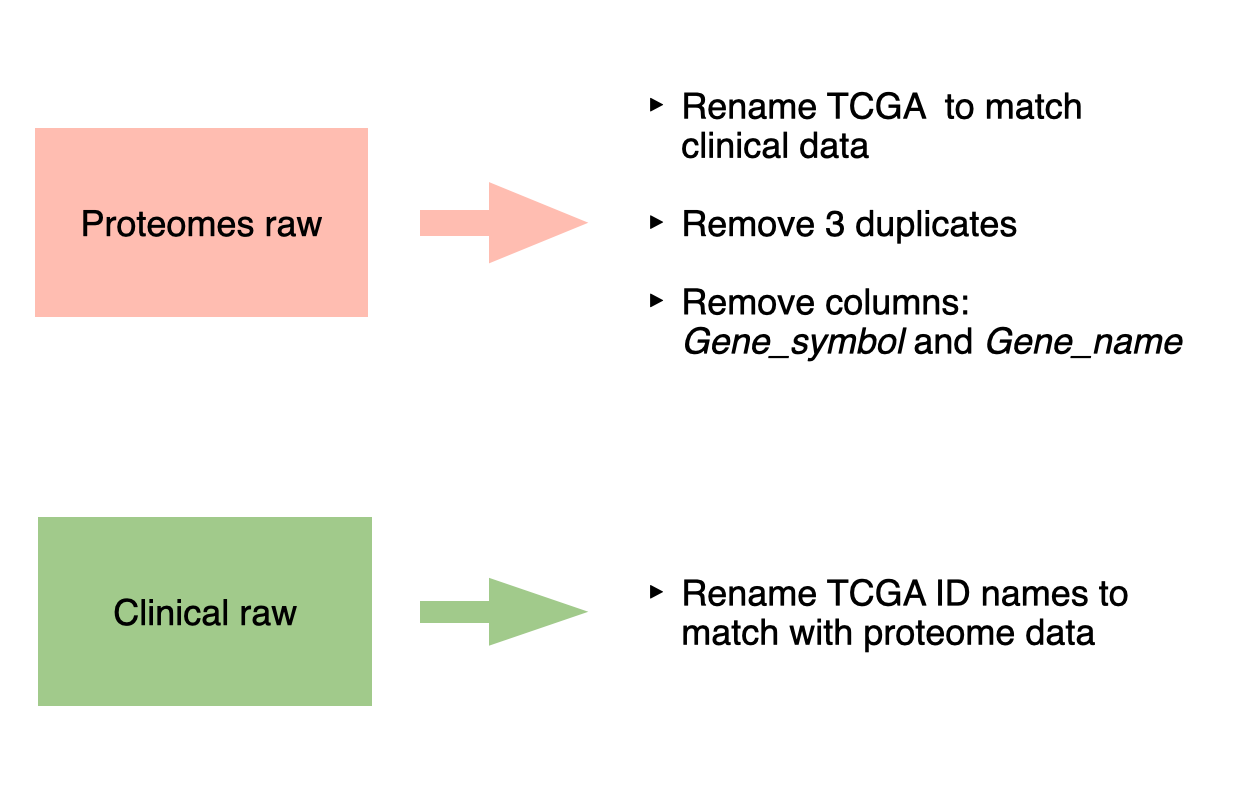
\includegraphics[width=7.29167in,height=\textheight]{/cloud/project/results/workflowClean.png}
\end{frame}

\begin{frame}{Augmenting data}
\protect\hypertarget{augmenting-data}{}
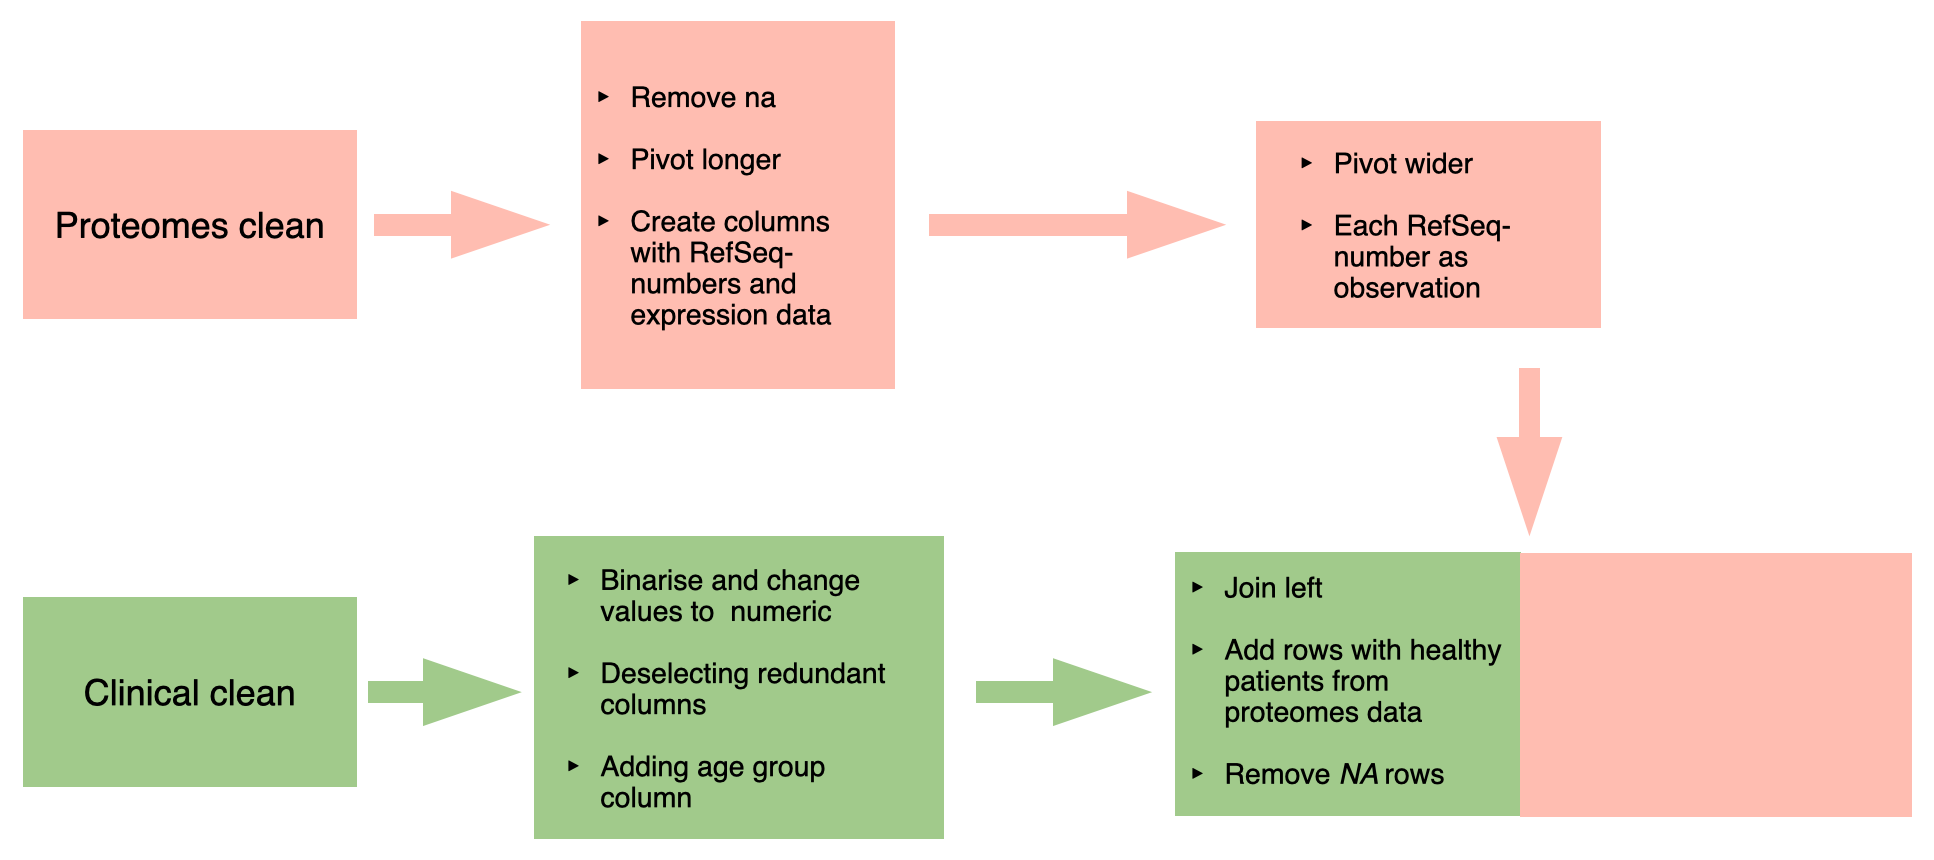
\includegraphics[width=8.33333in,height=\textheight]{/cloud/project/results/WorkflowAugment.png}
\end{frame}

\hypertarget{results}{%
\section{Results}\label{results}}

\begin{frame}{Cancer sub-types in each age group}
\protect\hypertarget{cancer-sub-types-in-each-age-group}{}
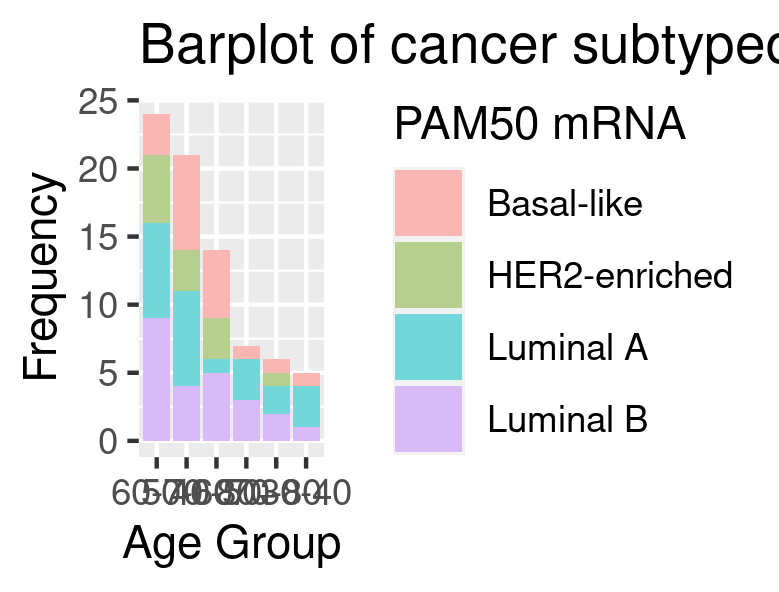
\includegraphics[width=8.33333in,height=\textheight]{/cloud/project/results/barPlotcancersubtypedPAM50.png}

\textbf{PAM50 test} usually categorizes cancer into 5 sub-types. But in
our dataset, we found 4 sub-types only and we stuck to it.
\end{frame}

\begin{frame}{No.~of tumors per cancer stage}
\protect\hypertarget{no.-of-tumors-per-cancer-stage}{}
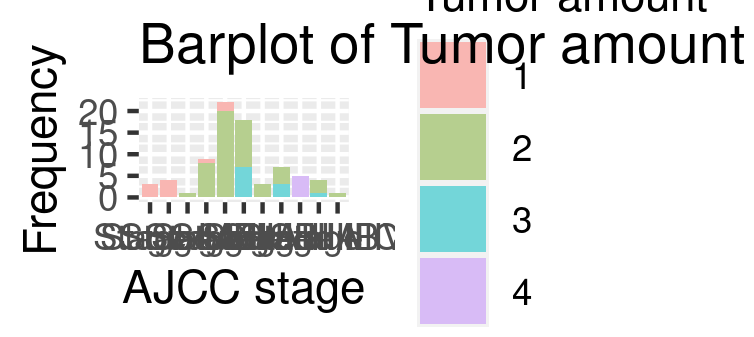
\includegraphics[width=8.33333in,height=\textheight]{/cloud/project/results/barPlotAJCCTumorAmount.png}

\textbf{AJCC staging system}: American Joint Committee on Cancer's
system to describe the amount and spread of cancer
\end{frame}

\begin{frame}{Expression level variation - for review}
\protect\hypertarget{expression-level-variation---for-review}{}
\includegraphics[width=0.49\linewidth,height=0.6\textheight]{../results/heatmapPAM50}
\includegraphics[width=0.49\linewidth,height=0.6\textheight]{../results/heatmapTumor}
\end{frame}

\begin{frame}{Expression level variation - for review}
\protect\hypertarget{expression-level-variation---for-review-1}{}
\begin{longtable}[]{@{}
  >{\raggedright\arraybackslash}p{(\columnwidth - 2\tabcolsep) * \real{0.5000}}
  >{\raggedright\arraybackslash}p{(\columnwidth - 2\tabcolsep) * \real{0.5000}}@{}}
\toprule
\endhead
\includegraphics[width=3.4375in,height=\textheight]{/cloud/project/results/heatmapPAM50.png}
&
\includegraphics[width=3.29167in,height=\textheight]{/cloud/project/results/heatmapTumor.png} \\
\bottomrule
\end{longtable}
\end{frame}

\begin{frame}{Principal components and k-means clusters - for review}
\protect\hypertarget{principal-components-and-k-means-clusters---for-review}{}
\includegraphics[width=0.45\linewidth,height=0.45\textheight]{../results/pcaRotationMatrix}
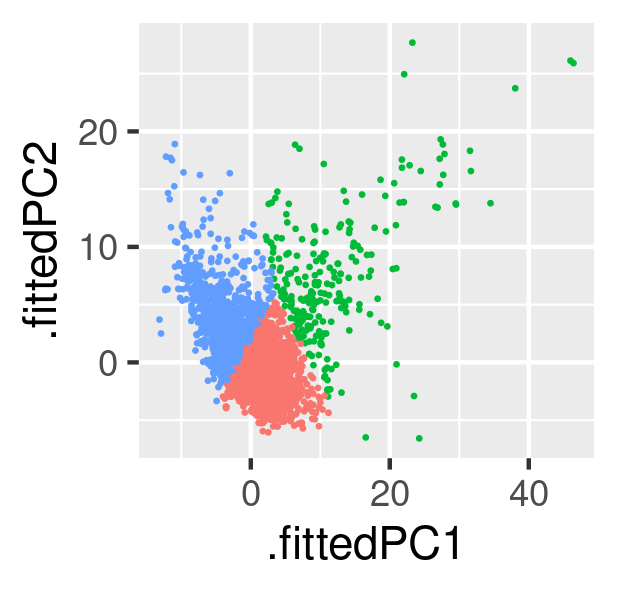
\includegraphics[width=0.45\linewidth,height=0.45\textheight]{../results/kplot1}
\end{frame}

\begin{frame}{Principal components and k-means clusters - for review}
\protect\hypertarget{principal-components-and-k-means-clusters---for-review-1}{}
\begin{longtable}[]{@{}
  >{\raggedright\arraybackslash}p{(\columnwidth - 2\tabcolsep) * \real{0.5462}}
  >{\raggedright\arraybackslash}p{(\columnwidth - 2\tabcolsep) * \real{0.4538}}@{}}
\toprule
\endhead
\includegraphics[width=3.4375in,height=\textheight]{/cloud/project/results/pcaRotationMatrix.png}
&
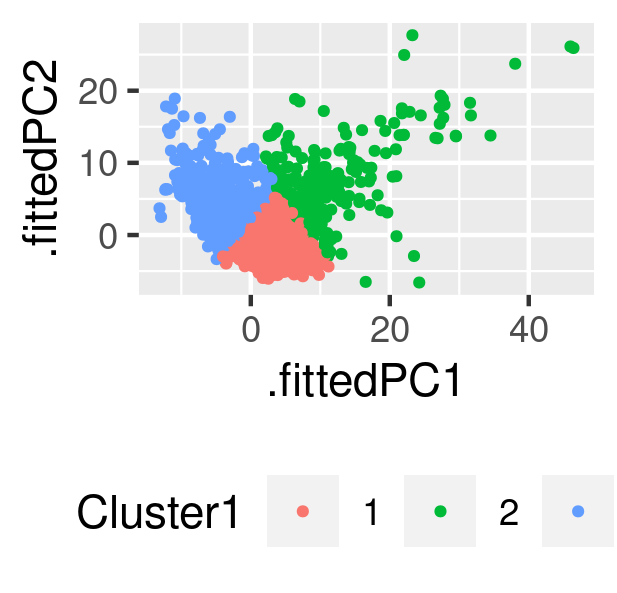
\includegraphics[width=3.29167in,height=\textheight]{/cloud/project/results/kplot1.png} \\
\bottomrule
\end{longtable}
\end{frame}

\begin{frame}{Discussion}
\protect\hypertarget{discussion}{}
1. How different is the data for healthy individuals from unhealthy
individuals?

2. Can we target unhealthy individuals with specific but different
medicines in line with which cluster they are a part of?
\end{frame}

\end{document}
